Sur la carte, le joueur utilise les flèches du clavier pour se déplacer. Il peut aller dans quatre directions :

\begin{itemize}
    \item à droite:
          \begin{figure}[H]
              \centering
              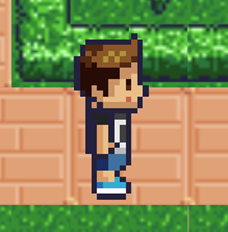
\includegraphics[width=0.1\textwidth ]{images/movements/playerRight.png}
              \caption{Mouvement du joueur à droite}
              \label{fig:pic_dessus}
          \end{figure}

    \item à gauche:
          \begin{figure}[H]
              \centering
              \includegraphics[width=0.1\textwidth ]{images/movements/playerLeft.png}
              \caption{Mouvement du joueur à gauche}
              \label{fig:pic_dessus}
          \end{figure}

    \item en bas:
          \begin{figure}[H]
              \centering
              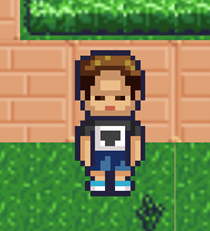
\includegraphics[width=0.1\textwidth ]{images/movements/playerDown.png}
              \caption{Mouvement du joueur en bas}
              \label{fig:pic_dessus}
          \end{figure}

    \item en haut:
          \begin{figure}[H]
              \centering
              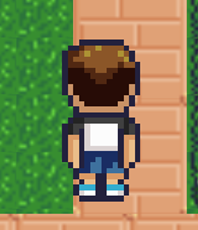
\includegraphics[width=0.1\textwidth ]{images/movements/playerUp.png}
              \caption{Mouvement du joueur en haut}
              \label{fig:pic_dessus}
          \end{figure}
\end{itemize}


Le joueur ne peut pas se déplacer partout! Lorsque qu'il rencontre un obstacle il est bloqué et ne peut pas passer par dessus.